\chapter{Cor e absorbância}\label{ch:g11:absorbance}

Uma garrafa de bebida isotônica brilha num azul intenso no banco de uma
academia. A sua cor vem de um corante dissolvido nela, alguns
miligramas num litro inteiro: pouco demais para pesar, e pouco demais
para ver como sólido. Mesmo assim, um laboratório de alimentos precisa
verificar essa quantidade, porque um corante só pode ser acrescentado
dentro de certos limites. A própria cor é a chave. Quanto mais corante
uma solução contém, mais luz ela absorve; um instrumento que mede quanta
luz uma solução absorve mede, na verdade, uma concentração.

\begin{recall}
As \omterm{def:g10:concentration-and-dilution:mass-concentration}{concentrações em massa} e molar de uma solução; a \omterm{def:g10:concentration-and-dilution:dilution}{diluição} de uma
\omterm{def:g10:concentration-and-dilution:dilution}{solução-estoque}; uma \omterm{def:g10:concentration-and-dilution:standard}{escala de padrões} comparada com uma solução
desconhecida (\cref{ch:g10:concentration-and-dilution}).
\end{recall}

\begin{omfigure}
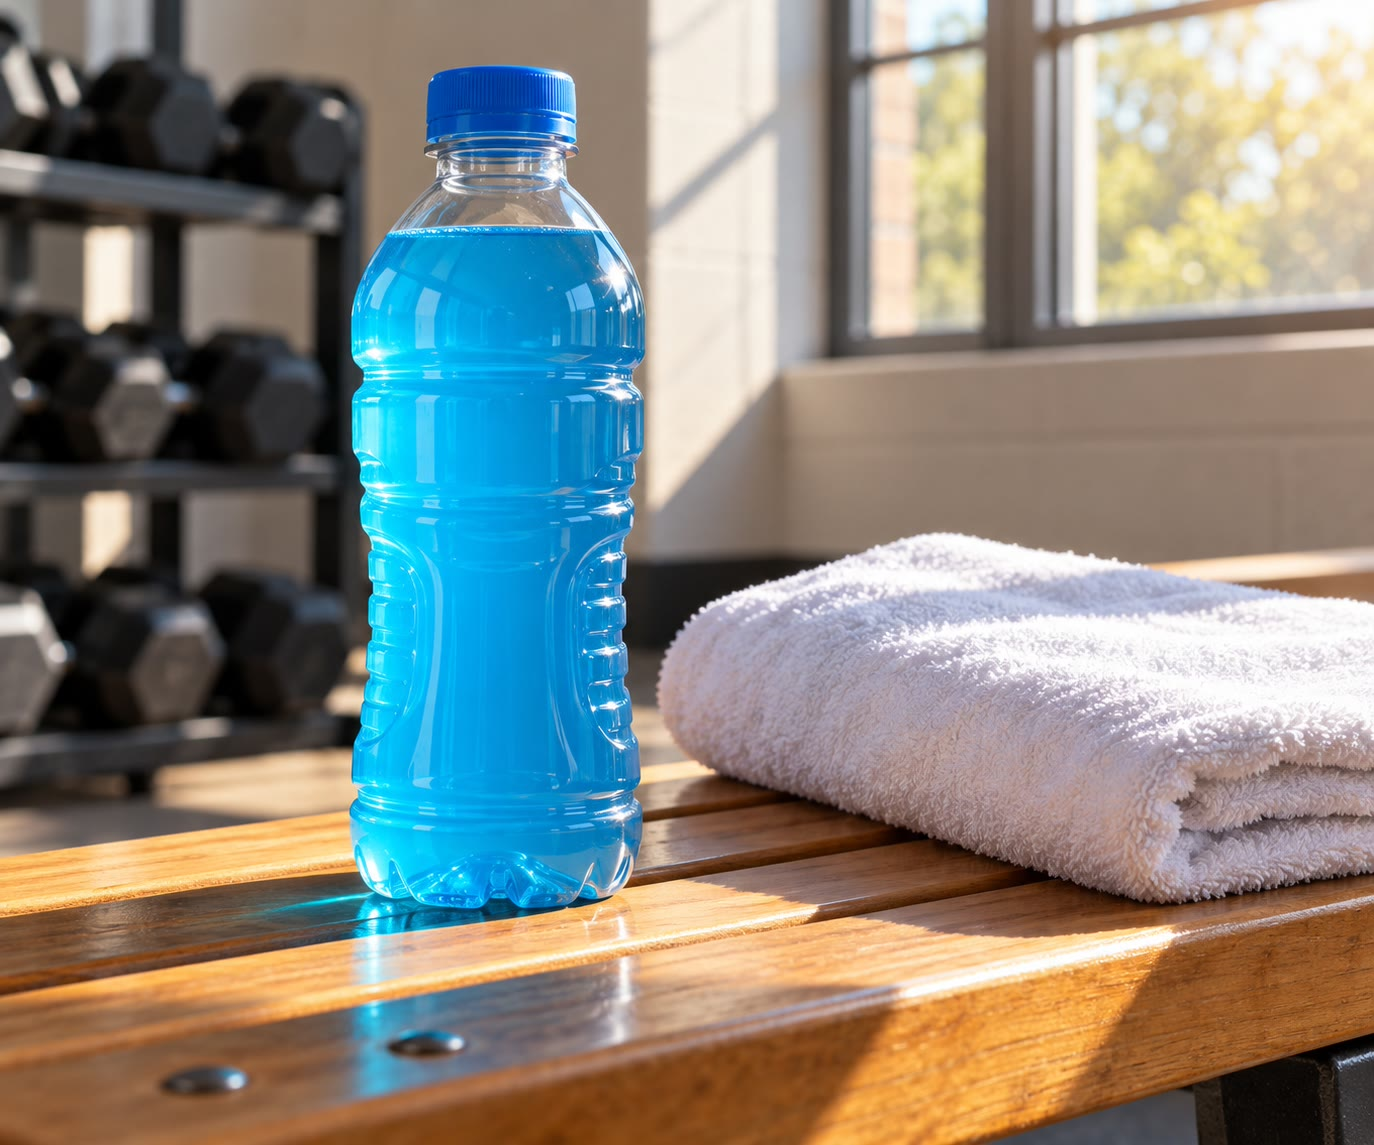
\includegraphics[width=0.5\linewidth]{images/book1/ai/g11-sports-drink.jpg}

{\small Uma bebida azul: a sua cor vem de alguns miligramas de corante
por litro.}
\end{omfigure}

\section{A cor de uma solução}

A luz branca, como a luz do dia, é uma \omterm{def:g6:pure-substances-and-mixtures:mixture}{mistura} de todas as cores do
arco-íris. Cada cor corresponde a um comprimento de onda, de cerca de
\qty{400}{nm} para o violeta a cerca de \qty{750}{nm} para o vermelho; o
livro de física explica o que é um comprimento de onda, e aqui ele é
só um rótulo para uma cor. Uma solução colorida absorve uma parte da luz
que a atravessa, algumas cores muito mais que outras; o olho vê as cores
que passam.

\begin{definition}[Cores complementares]\label{def:g11:absorbance:complementary}
Duas cores são \emph{cores complementares}\index{cores complementares}
se a \omterm{def:g6:pure-substances-and-mixtures:mixture}{mistura} delas dá luz branca. Num círculo cromático, as cores
complementares ficam uma diante da outra.
\end{definition}

\begin{omfigure}
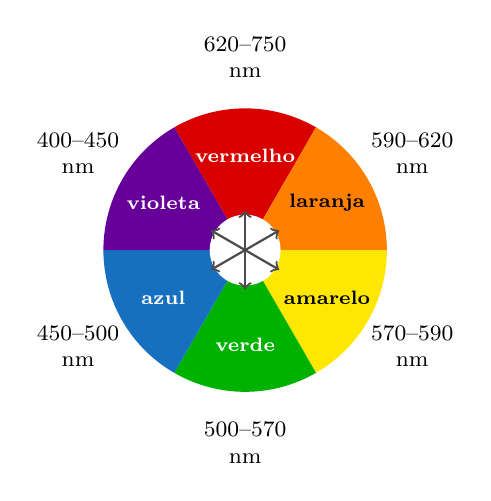
\begin{tikzpicture}[font=\small]
  \foreach \a/\c/\n/\w/\t in {90/red!85!black/{\scriptsize vermelho}/{620--750}/white,
      30/orange/{\scriptsize laranja}/{590--620}/black, -30/yellow!90!orange/{\scriptsize amarelo}/{570--590}/black,
      -90/green!70!black/{\scriptsize verde}/{500--570}/white, -150/cyan!50!blue/{\scriptsize azul}/{450--500}/white,
      150/violet!80!blue/{\scriptsize violeta}/{400--450}/white} {
    \fill[\c] (0,0) -- (\a-30:1.8) arc[start angle=\a-30, end angle=\a+30,
      radius=1.8] -- cycle;
    \node[text=\t, font=\small\bfseries] at (\a:1.2) {\n};
    \node[font=\footnotesize, align=center] at (\a:2.45) {\w\\ nm};
  }
  \fill[white] (0,0) circle (0.45);
  \draw[<->, thick, black!70] (90:0.5) -- (-90:0.5);
  \draw[<->, thick, black!70] (30:0.5) -- (-150:0.5);
  \draw[<->, thick, black!70] (-30:0.5) -- (150:0.5);
\end{tikzpicture}

{\small Um círculo cromático, com comprimentos de onda aproximados. As
\omterm{def:g11:absorbance:complementary}{cores complementares} ficam uma diante da outra: vermelho e verde,
laranja e azul, amarelo e violeta.}
\end{omfigure}

\begin{proposition}[A cor vista]\label{prop:g11:absorbance:colour-seen}
Uma solução que absorve principalmente uma cor da luz branca tem a cor
complementar dessa cor.
\end{proposition}

\begin{proof}
Admitido: a luz que passa é a luz branca menos a cor absorvida, e o olho
vê esse resto como a cor complementar.
\end{proof}

\begin{example}[Dois corantes alimentares]\label{ex:g11:absorbance:dyes}
% ledger: lmax:E133, lmax:E102
O corante azul da bebida isotônica, conhecido como azul brilhante
(E133), absorve principalmente a luz vermelho-alaranjada, por volta de
\qty{629}{nm}: ele parece azul. O corante amarelo tartrazina (E102)
absorve principalmente a luz azul-violeta, por volta de \qty{427}{nm}:
ele parece amarelo. Uma bebida verde em geral contém os dois.
\end{example}

\section{O espectro de absorção}

\begin{definition}[Espectro de absorção]\label{def:g11:absorbance:spectrum}
O \emph{espectro de absorção}\index{espectro de absorcao@espectro de absorção} de uma solução
é o gráfico da luz que ela absorve (a sua \omterm{def:g11:absorbance:absorbance}{absorbância}, definida na seção
seguinte) em função do comprimento de onda. O comprimento de onda em que
a absorção é maior é representado por $\lambda_{\max}$.
\end{definition}

\begin{omfigure}
\begin{tikzpicture}
\begin{axis}[width=0.85\linewidth, height=6cm, xmin=380, xmax=750,
    ymin=0, ymax=0.95, xlabel={comprimento de onda $\lambda$ (\si{nm})},
    ylabel={absorbância $A$}, axis lines*=left, ymajorgrids,
    grid style={gray!20}, tick label style={font=\small},
    label style={font=\small}, xtick={400,450,500,550,600,650,700,750},
    ]
  % ledger: lmax:E133, abs:E133, lmax:E102, abs:E102 (band shapes synthetic)
  \addplot[very thick, cyan!60!blue] table[x=lambda, y=E133]
    {figdata/out/grade-11-absorbance-a.dat};
  \addplot[very thick, orange!85!yellow] table[x=lambda, y=E102]
    {figdata/out/grade-11-absorbance-a.dat};
  \node[font=\small, align=left, anchor=west, text=cyan!60!blue!80!black]
    at (axis cs:668,0.62) {E133 (azul),\\ \qty{5.0}{mg/L}};
  \node[font=\small, align=left, anchor=west, text=orange!80!black]
    at (axis cs:470,0.66) {E102 (amarelo),\\ \qty{15}{mg/L}};
  \addplot[dashed, black!50] coordinates {(629,0) (629,0.82)};
  \addplot[dashed, black!50] coordinates {(427,0) (427,0.795)};
  \node[font=\small, anchor=south] at (axis cs:629,0.83) {\qty{629}{nm}};
  \node[font=\small, anchor=south] at (axis cs:427,0.81) {\qty{427}{nm}};
\end{axis}
\end{tikzpicture}

{\small \omterm{def:g11:absorbance:spectrum}{Espectros de absorção} dos dois corantes em água, numa cubeta de
\qty{1}{cm} de espessura. As formas das bandas foram desenhadas a partir
de um modelo simples; as posições dos máximos e as suas alturas são as
das especificações dos dois corantes.}
\end{omfigure}

\begin{remark}[Ler um espectro]\label{rem:g11:absorbance:reading}
O corante azul quase não absorve nada abaixo de \qty{520}{nm}: a luz
azul e a violeta passam, e a solução parece azul. O corante amarelo
quase não absorve nada acima de \qty{520}{nm}: a luz verde, a amarela, a
laranja e a vermelha passam, e o olho vê amarelo. A \qty{629}{nm}, só o
corante azul absorve; a \qty{427}{nm}, quase só o amarelo.
\end{remark}

\section{A absorbância e o espectrofotômetro}

\begin{definition}[Absorbância]\label{def:g11:absorbance:absorbance}
A \emph{absorbância}\index{absorbancia@absorbância} $A$ de uma solução, num
comprimento de onda escolhido, é o número mostrado por um
espectrofotômetro que mede quanto da luz desse comprimento de onda a
solução absorve. Ela não tem unidade; ela é zero para o \omterm{def:g6:solutions-and-solubility:solute}{solvente} puro, e
tanto maior quanto mais luz a solução absorve.
\end{definition}

\begin{omfigure}
\begin{tikzpicture}[font=\small]
  % lamp
  \shade[ball color=yellow!40] (0,0.6) circle (0.32);
  \foreach \a in {0,45,90,135,180,225,270,315} \draw[yellow!60!orange, thick] (\a:0.4) ++(0,0.6) -- ++(\a:0.18);
  \node[anchor=north] at (0,-0.25) {lâmpada};
  \draw[black!60, thick] (0.8,0.6) -- (1.75,0.6);
  % prism
  \fill[cyan!10, draw=black!60] (1.75,0.15) -- (2.55,0.15) -- (2.15,1.15) -- cycle;
  \node[anchor=north] at (2.15,-0.25) {prisma};
  \foreach \c/\d in {violet/0.35, blue/0.22, green!70!black/0.08, yellow!90!orange/-0.06,
      orange/-0.2, red/-0.34}
    \draw[\c, thick] (2.45,0.6) -- (3.45,{0.6+\d});
  % slit
  \fill[black!70] (3.5,0.92) rectangle (3.6,1.4);
  \fill[black!70] (3.5,-0.2) rectangle (3.6,0.52);
  \node[anchor=north] at (3.55,-0.25) {fenda};
  \draw[orange, very thick] (3.6,0.6) -- (4.75,0.6);
  % cuvette
  \pic (cv) at (5,0) {cuvette={0.75}{cyan!50!blue!45}};
  \node[anchor=north] at (5,-0.25) {cubeta};
  \draw[orange!60, thick] (5.3,0.6) -- (6.3,0.6);
  % detector and display
  \fill[black!15, draw=black!60] (6.3,0.2) rectangle (6.9,1.0);
  \node[anchor=north] at (6.6,-0.25) {detector};
  \draw[black!60] (6.9,0.6) -- (7.4,0.6);
  \fill[black!80, draw=black] (7.4,0.25) rectangle (9.4,0.95);
  \node[green!70!white, font=\footnotesize\ttfamily] at (8.4,0.6) {A = 0.590};
  \node[anchor=north] at (8.4,-0.25) {visor};
\end{tikzpicture}

{\small Princípio de um espectrofotômetro. Um prisma separa a luz branca
nas suas cores; uma fenda deixa passar só um comprimento de onda,
escolhido pelo usuário; o detector compara a luz que sai da cubeta com
a luz que entra nela, e o visor dá a \omterm{def:g11:absorbance:absorbance}{absorbância}.}
\end{omfigure}

\begin{remark}[De onde vem o número]\label{rem:g11:absorbance:log}
A \omterm{def:g11:absorbance:absorbance}{absorbância} é calculada pelo instrumento a partir das intensidades da
luz que entra na solução e que sai dela, com uma função matemática vista
no último ano da escola, o logaritmo. Um volume universitário dá a
fórmula; aqui, a \omterm{def:g11:absorbance:absorbance}{absorbância} é simplesmente o que o instrumento lê.
\end{remark}

\begin{inthelab}[Zerar o espectrofotômetro]
A cubeta, o \omterm{def:g6:solutions-and-solubility:solute}{solvente} e o próprio instrumento absorvem um pouco de luz.
Antes de qualquer medida, uma cubeta cheia do \omterm{def:g6:solutions-and-solubility:solute}{solvente} puro, o
\emph{branco}, é colocada no instrumento, que é ajustado para ler
$A = 0$ no comprimento de onda escolhido. Cada leitura que vem depois é
a \omterm{def:g11:absorbance:absorbance}{absorbância} do \omterm{def:g6:solutions-and-solubility:solute}{soluto} sozinho. As cubetas são sempre seguradas pelas
faces foscas, e limpas: uma impressão digital numa face transparente
também absorve luz.
\end{inthelab}

\begin{omfigure}
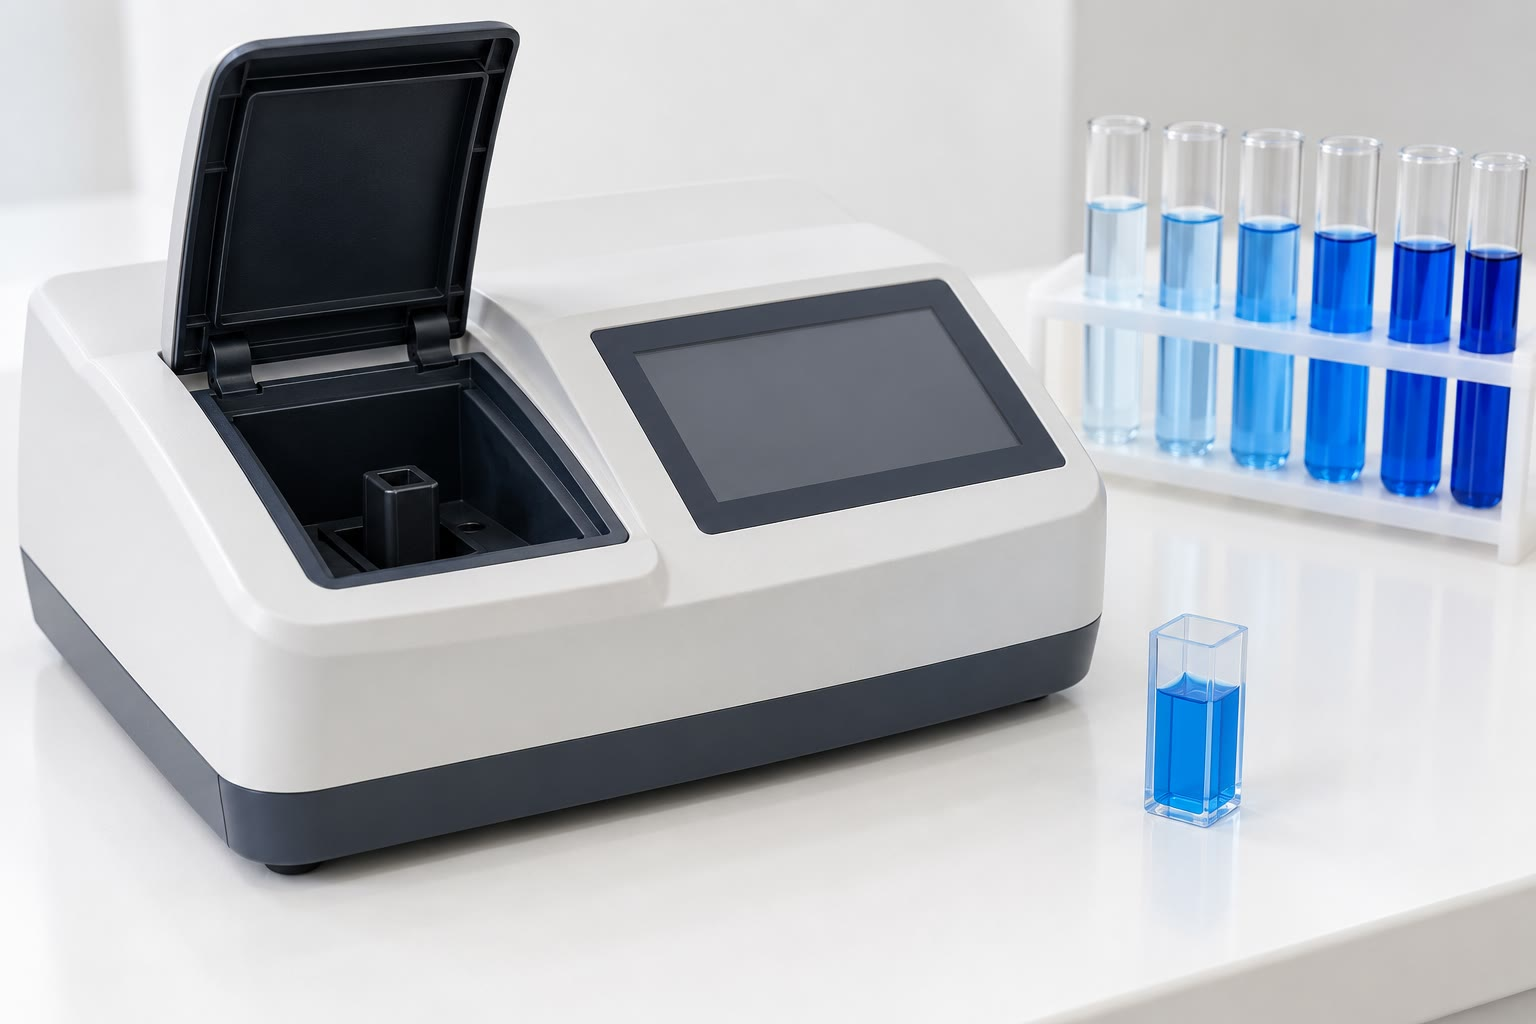
\includegraphics[width=0.5\linewidth]{images/book1/ai/g11-spectrophotometer.jpg}

{\small Um espectrofotômetro e as suas cubetas quadradas.}
\end{omfigure}

\section{A lei de Beer--Lambert}

\begin{definition}[Coeficiente de absorção molar]\label{def:g11:absorbance:epsilon}
O \emph{coeficiente de absorção molar}\index{coeficiente de absorcao molar@coeficiente de absorção molar}
$\varepsilon$ de uma espécie dissolvida, num dado comprimento de onda,
mede com que intensidade um \omterm{def:g10:the-mole:amount}{mol} dela absorve a luz; ele depende da
espécie, do \omterm{def:g6:solutions-and-solubility:solute}{solvente} e do comprimento de onda, e é expresso em
\si{L/(mol.cm)}.
\end{definition}

\begin{proposition}[Lei de Beer--Lambert]\label{prop:g11:absorbance:beer-lambert}
Para uma solução diluída de uma única espécie absorvente, de
\omterm{def:g10:concentration-and-dilution:molar-concentration}{concentração molar} $c$, numa cubeta de espessura $\ell$, a \omterm{def:g11:absorbance:absorbance}{absorbância}
num dado comprimento de onda é
\[
  A = \varepsilon\, \ell\, c .
\]
A \omterm{def:g11:absorbance:absorbance}{absorbância} é proporcional à concentração.
\end{proposition}

\begin{proof}
Admitida aqui; ela é demonstrada num volume universitário.
\end{proof}


\begin{remark}[Com uma concentração em massa]\label{rem:g11:absorbance:mass}
% ledger: abs:E133, mw:E133
Como $c = C_m / M$, a lei também pode ser escrita $A = a\, \ell\, C_m$,
com $a = \varepsilon / M$ em \si{L/(g.cm)}. As especificações dos
corantes alimentares dão $a$: para o corante azul E133 a \qty{629}{nm},
$a =
\qty{164}{L/(g.cm)}$, e com a sua \omterm{def:g10:the-mole:molar-mass}{massa molar} de \qty{792.9}{g/mol},
$\varepsilon = 164 \times 792.9 = \qty{1.30e5}{L/(mol.cm)}$. Uma solução
de só \qty{5.0}{mg/L} dele, numa cubeta de \qty{1}{cm}, já lê
$A = 164 \times 1 \times 0.0050 = 0.82$.
\end{remark}

\begin{remark}[Só soluções diluídas]\label{rem:g11:absorbance:dilute}
A proporcionalidade só vale para soluções diluídas, na prática para
\omterm{def:g11:absorbance:absorbance}{absorbâncias} abaixo de cerca de 1 a 1.5 num instrumento comum. Uma
solução concentrada demais é diluída por um fator conhecido antes de ser
medida.
\end{remark}
\section{Medir uma concentração}

\begin{definition}[Reta de calibração]\label{def:g11:absorbance:calibration-line}
Uma \emph{reta de calibração}\index{reta de calibracao@reta de calibração} é o gráfico da
\omterm{def:g11:absorbance:absorbance}{absorbância} de uma série de \omterm{def:g10:concentration-and-dilution:standard}{soluções-padrão} de uma mesma espécie,
medidas no mesmo comprimento de onda e na mesma cubeta, em função da sua
concentração. Quando a lei de Beer--Lambert vale, ela é uma reta que
passa pela origem.
\end{definition}

\begin{method}[Medir uma concentração com uma reta de calibração]\label{met:g11:absorbance:calibration}
\begin{enumerate}
  \item Registre o \omterm{def:g11:absorbance:spectrum}{espectro de absorção} da espécie e escolha o
        comprimento de onda $\lambda_{\max}$, em que a \omterm{def:g11:absorbance:absorbance}{absorbância} é
        maior e varia menos com um pequeno erro no comprimento de onda.
  \item Zere o instrumento com o branco.
  \item Prepare \omterm{def:g10:concentration-and-dilution:standard}{soluções-padrão} por \omterm{def:g10:concentration-and-dilution:dilution}{diluição} de uma \omterm{def:g10:concentration-and-dilution:dilution}{solução-estoque} e
        meça as suas \omterm{def:g11:absorbance:absorbance}{absorbâncias}.
  \item Trace $A$ em função da concentração e desenhe a reta que passa
        pela origem mais próxima dos pontos.
  \item Meça a solução desconhecida, diluída se necessário para que a
        sua \omterm{def:g11:absorbance:absorbance}{absorbância} fique entre as dos padrões, e leia a sua
        concentração na reta (ou divida $A$ pelo coeficiente angular);
        multiplique pelo \omterm{def:g10:concentration-and-dilution:dilution}{fator de diluição}.
\end{enumerate}
\end{method}

\begin{omfigure}
\begin{tikzpicture}
\begin{axis}[width=0.72\linewidth, height=6cm, xmin=0, xmax=5.6,
    ymin=0, ymax=0.95, xlabel={concentração de E133 (\si{mg/L})},
    ylabel={absorbância a \qty{629}{nm}}, axis lines*=left, ymajorgrids,
    xmajorgrids, grid style={gray!20}, tick label style={font=\small},
    label style={font=\small}]
  % ledger: abs:E133 (points synthetic: exact values + fixed offsets)
  \addplot[only marks, mark=*, mark size=2.2pt, omDef] table[x=C, y=A]
    {figdata/out/grade-11-absorbance-b.dat};
  \addplot[thick, omProp, domain=0:5.5] {0.164*x};
  \addplot[dashed, black!60] coordinates {(0,0.590) (3.6,0.590) (3.6,0)};
  \node[font=\small, anchor=south west] at (axis cs:0.1,0.6) {desconhecida: $A = 0.590$};
  \node[font=\small, anchor=west] at (axis cs:3.65,0.22) {\qty{3.6}{mg/L}};
\end{axis}
\end{tikzpicture}

{\small \omterm{def:g11:absorbance:calibration-line}{Reta de calibração} do corante azul: cinco padrões (pontos) e a
reta que passa pela origem, de coeficiente angular \qty{0.164}{L/mg}.
Uma solução desconhecida que lê $A = 0.590$ tem uma concentração de
$0.590 / 0.164 =
\qty{3.6}{mg/L}$.}
\end{omfigure}

\begin{example}[Os cinco padrões]\label{ex:g11:absorbance:standards}
Uma \omterm{def:g10:concentration-and-dilution:dilution}{solução-estoque} do corante azul a \qty{100}{mg/L} é diluída para dar
\qty{100.0}{mL} de cada padrão: para \qty{2.0}{mg/L}, o \omterm{def:g10:concentration-and-dilution:dilution}{fator de
diluição} é 50, então \qty{2.0}{mL} da \omterm{def:g10:concentration-and-dilution:dilution}{solução-estoque} são completados
até \qty{100.0}{mL}. Os cinco padrões, de 1 a \qty{5}{mg/L}, leem 0.168,
0.325, 0.494, 0.652 e 0.823: a poucos milésimos de $0.164 \times C$, a
reta da figura.
\end{example}

\section{Exercícios}

\begin{exercise}[$\star$]\label{exo:g11:absorbance:1}
Uma solução absorve principalmente a luz laranja. De que cor ela
parece? E uma solução que absorve principalmente a luz violeta?
\end{exercise}

\begin{exercise}[$\star$]\label{exo:g11:absorbance:2}
Usando o círculo cromático, dê a cor principalmente absorvida por uma
solução verde, e a faixa de comprimentos de onda que essa cor cobre.
\end{exercise}

\begin{exercise}[$\star$]\label{exo:g11:absorbance:3}
Leia nos \omterm{def:g11:absorbance:spectrum}{espectros de absorção} o comprimento de onda $\lambda_{\max}$
de cada corante e a sua \omterm{def:g11:absorbance:absorbance}{absorbância} nesse ponto.
\end{exercise}

\begin{exercise}[$\star$]\label{exo:g11:absorbance:4}
Uma solução de corante a \qty{2.0}{mg/L} lê $A = 0.30$. Quanto lê uma
solução do mesmo corante a \qty{6.0}{mg/L}, na mesma cubeta e no mesmo
comprimento de onda? E a \qty{1.0}{mg/L}?
\end{exercise}

\begin{exercise}[$\star$]\label{exo:g11:absorbance:5}
O que é o branco de um espectrofotômetro, e por que o instrumento é
zerado com ele?
\end{exercise}

\begin{exercise}[$\star\star$]\label{exo:g11:absorbance:6}
Usando a \omterm{def:g11:absorbance:calibration-line}{reta de calibração} do corante azul, encontre a concentração de
uma solução que lê $A = 0.41$.
\end{exercise}

\begin{exercise}[$\star\star$]\label{exo:g11:absorbance:7}
Para medir o corante azul, por que ajustar o espectrofotômetro em
\qty{629}{nm}, e não em \qty{550}{nm}? Dê duas razões.
\end{exercise}

\begin{exercise}[$\star\star$]\label{exo:g11:absorbance:8}
Uma bebida não diluída lê $A = 2.4$ a \qty{629}{nm}, alto demais para
merecer confiança. Ela é diluída cinco vezes e passa a ler $A = 0.48$.
Encontre a concentração de corante azul na bebida.
\end{exercise}

\begin{exercise}[$\star\star$]\label{exo:g11:absorbance:9}
% ledger: mw:E102, abs:E102
Uma solução de tartrazina a \qty{15.0}{mg/L} lê $A = 0.795$ a
\qty{427}{nm} numa cubeta de \qty{1.00}{cm}. Calcule a sua absortividade
$a$ em \si{L/(g.cm)}, e depois o seu \omterm{def:g11:absorbance:epsilon}{coeficiente de absorção molar}
(\omterm{def:g10:the-mole:molar-mass}{massa molar} \qty{534.4}{g/mol}).
\end{exercise}

\begin{exercise}[$\star\star$]\label{exo:g11:absorbance:10}
Olhe os espectros dos dois corantes. Acima de que comprimento de onda o
corante amarelo quase não absorve nada? Por que o corante azul pode ser
medido a \qty{629}{nm} mesmo numa bebida verde que também contém o
corante amarelo?
\end{exercise}

\begin{exercise}[$\star\star$]\label{exo:g11:absorbance:11}
A mesma solução é medida numa cubeta de \qty{2.0}{cm} de espessura em
vez de \qty{1.0}{cm}. Como a sua \omterm{def:g11:absorbance:absorbance}{absorbância} muda? Por quê?
\end{exercise}

\begin{exercise}[$\star\star\star$]\label{exo:g11:absorbance:12}
Padrões do corante azul a 5, 10, 20 e \qty{40}{mg/L} leem 0.82, 1.62,
2.30 e 2.70. Calcule $A / C$ para cada um. O que você observa? Que
padrões podem ser usados para uma \omterm{def:g11:absorbance:calibration-line}{reta de calibração}, e o que fazer com
uma solução desconhecida que lê $2.5$?
\end{exercise}

\begin{exercise}[$\star\star\star$]\label{exo:g11:absorbance:13}
Uma bebida verde contém o corante azul e o corante amarelo. Numa cubeta
de \qty{1.00}{cm}, ela lê $A = 0.574$ a \qty{629}{nm} e $A = 0.53$ a
\qty{427}{nm}. A \qty{427}{nm}, o corante azul quase não absorve nada,
e a \qty{629}{nm} o corante amarelo não absorve nada. Encontre as
\omterm{def:g10:concentration-and-dilution:mass-concentration}{concentrações em massa} dos dois corantes (use $a = \qty{164}{L/(g.cm)}$
e $a = \qty{53.0}{L/(g.cm)}$).
\end{exercise}

\begin{exercise}[$\star\star\star$]\label{exo:g11:absorbance:14}
Uma aluna esquece o branco e zera o instrumento com uma cubeta vazia.
Todas as leituras ficam então \num{0.040} altas demais. A solução
desconhecida lê $0.368$, e ela divide pelo coeficiente angular $0.164$
da \omterm{def:g11:absorbance:calibration-line}{reta de calibração} verdadeira. Que concentração ela encontra? Qual é
a verdadeira? Em que porcentagem ela erra?
\end{exercise}

\begin{exercise}[$\star\star\star$]\label{exo:g11:absorbance:15}
% ledger: adi:E102
A ingestão diária aceitável de tartrazina é de \qty{10}{mg} por
quilograma de massa corporal. Uma bebida contém \qty{20}{mg/L} dela. Que
volume da bebida levaria um adulto de \qty{60}{kg} a essa ingestão num
dia? Esse é um risco realista?
\end{exercise}

\section{Problema: o azul de uma bebida isotônica}


\begin{problem}[{Problema de fim de semana --- quantas garrafas de uma
bebida isotônica azul uma criança teria de beber para chegar ao limite
diário seguro do seu corante?}]
\label{pb:g11:absorbance:1}
% ledger: lmax:E133, abs:E133, mw:E133, adi:E133
Um laboratório de alimentos verifica o corante azul E133 de uma bebida
isotônica vendida em garrafas de \qty{500}{mL}. As especificações do
corante dão a sua \omterm{def:g10:the-mole:molar-mass}{massa molar}, \qty{792.9}{g/mol}, e a sua ingestão
diária aceitável: \qty{6}{mg} por quilograma de massa corporal e por
dia, uma quantidade que pode ser ingerida todos os dias durante a vida
inteira sem risco apreciável.

\medskip
\noindent\textbf{Parte I --- Cor e espectro.}
\begin{enumerate}
  \item A bebida parece azul. Usando o círculo cromático, que cor de luz
        ela absorve mais?
  \item Leia o comprimento de onda $\lambda_{\max}$ do corante no seu
        espectro.
  \item Por que a \omterm{def:g11:absorbance:absorbance}{absorbância} do corante é quase zero a \qty{450}{nm}?
        Isso é coerente com a sua cor?
  \item Em que comprimento de onda as medidas devem ser feitas?
\end{enumerate}

\medskip
\noindent\textbf{Parte II --- A \omterm{def:g11:absorbance:calibration-line}{reta de calibração}.}
\begin{enumerate}[resume]
  \item Dissolvem-se \qty{50.0}{mg} de corante puro para fazer
        \qty{500.0}{mL} de \omterm{def:g10:concentration-and-dilution:dilution}{solução-estoque}. Calcule a sua \omterm{def:g10:concentration-and-dilution:mass-concentration}{concentração
        em massa} em \si{mg/L}.
  \item Fazem-se padrões de 1.0, 2.0, 3.0, 4.0 e \qty{5.0}{mg/L},
        \qty{100.0}{mL} de cada. Que volume de \omterm{def:g10:concentration-and-dilution:dilution}{solução-estoque} é
        necessário para o padrão de \qty{3.0}{mg/L}? Com que vidraria?
  \item Os padrões leem 0.168, 0.325, 0.494, 0.652 e 0.823. Calcule
        $A / C$ para cada um, e mostre que os pontos ficam perto de uma
        reta que passa pela origem, de coeficiente angular cerca de
        \qty{0.164}{L/mg}.
  \item Por que a reta tem de passar pela origem?
  \item Deduza a absortividade $a$ do corante em \si{L/(g.cm)} (cubeta
        de \qty{1.00}{cm}), e depois o seu \omterm{def:g11:absorbance:epsilon}{coeficiente de absorção molar}.
\end{enumerate}

\medskip
\noindent\textbf{Parte III --- A bebida.}
\begin{enumerate}[resume]
  \item \qty{25.0}{mL} de bebida são completados até \qty{50.0}{mL} com
        água. Qual é o \omterm{def:g10:concentration-and-dilution:dilution}{fator de diluição}?
  \item A bebida diluída lê $A = 0.590$. Encontre a sua concentração de
        corante.
  \item Deduza a concentração de corante na própria bebida.
  \item Quanto leria a bebida não diluída? Por que ela foi diluída?
  \item Calcule a massa de corante numa garrafa.
  \item Calcule a quantidade de corante, em \omterm{def:g10:the-mole:amount}{mols}, numa garrafa.
\end{enumerate}

\medskip
\noindent\textbf{Parte IV --- A ingestão diária aceitável.}
\begin{enumerate}[resume]
  \item Que massa do corante uma criança de \qty{30}{kg} pode ingerir
        por dia?
  \item Quantas garrafas a criança teria de beber num dia para chegar a
        esse valor?
  \item Que volume de bebida é esse? Comente.
  \item Mesma pergunta para um adulto de \qty{70}{kg}.
  \item Dê a resposta final: quantas garrafas de \qty{500}{mL} uma
        criança de \qty{30}{kg} teria de beber num dia para chegar à
        ingestão diária aceitável do corante?
\end{enumerate}
\end{problem}
